\documentclass{presentation}

\begin{document}

\begin{frame}
    \titlepage
\end{frame}

\begin{frame}{Übersicht}
    \tableofcontents
\end{frame}

\section{Einführung}

\begin{frame}[allowframebreaks]
	\frametitle{Motivation}
	Understanding program behavior is critical to overcome the expected architectural and programming complexities, such as limited power budgets, heterogeneity, hierarchical memories [...] We need new automatic analysis and \textbf{visualization} approaches to help application developers intuitively understand the multiple, interdependent effects that algorithmic choices have on application correctness or performance \cite{protools20}.
	\bibliographystyle{amsalpha}
	\bibliography{main.bib}
\end{frame}

\begin{frame}{Aufgabe}
    \begin{itemize}
        \item Programm entwickeln, zur Visualisierung komplexer paralleler Berechnungen auf CPUs und GPUs.
        \item Soll konfigurierbar sein.
        \item Soll 1 bis 3 dimensionale Berechnungen visualisieren können.
        \item Soll mit kleinen und großen Eingabedaten funktionieren.
        \item \underline{Einheitlich:} Visualisierung von MDHs, da diese komplexe Parallele-Berechnungen widerspiegeln können, u.a. auch die verwandter Arbeiten (durch geeignete Wahl von Tuning-Parametern)
    \end{itemize}
\end{frame}

\begin{frame}{Projektstruktur}
    \begin{figure}
        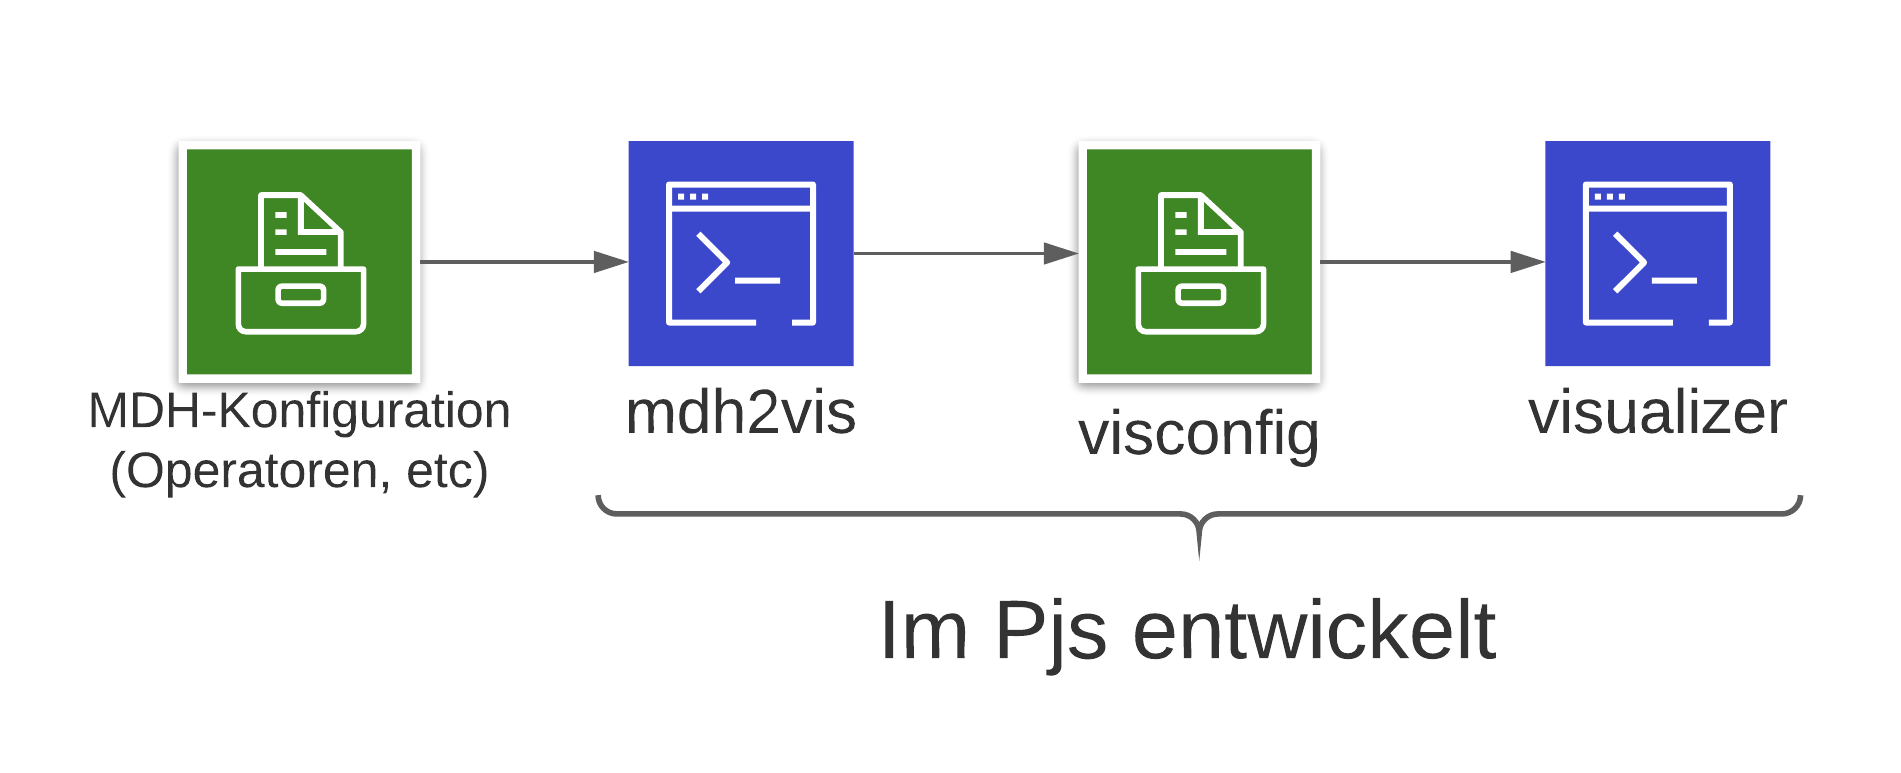
\includegraphics[scale=0.5]{struktur.png}
    \end{figure}
    
    \begin{itemize}
        \item Unterteilung in mehrere Projekte
            \begin{itemize}
                \item mdh2vis: Verarbeitet die MDH.
                \item visconfig: Spezifikation der Konfiguration des Visualisierungstools.
                \item visualizer: Visualisierungstool.
            \end{itemize}
    \end{itemize}
\end{frame}
\begin{frame}{OpenGL}
    \begin{itemize}
        \item API-Spezifikation entwickelt von Khronos Grop.
        \item Wird vom Betriebssystem oder vom GPU-Treiber implementiert.
        \item Bietet eine Schnittstelle, um Grafiken zu zeichnen.
        \item Verwendet typischerweise die GPU.
        \item Die Ausgabe kann mittels Shader (Programme die von OpenGL aufgerufen werden) angepasst werden.
        \item Definiert mehrere Typen von Buffer:
        \begin{itemize}
            \item VAO oder Mesh: Beschreibt etwas das gezeichnet werden sollt.
            \item Texture: Generischer Buffer. Typischerweise verwendet, um Bilder zu speichern.
            \item Renderbuffer: Interner Buffer.
            \item Framebuffer: Ausgabe-Buffer. Besteht aus Texturen und Renderbuffer.
        \end{itemize}
        \item Zeichnen: Mesh und Framebuffer anbinden und Shader ausführen.
    \end{itemize}
\end{frame}

\begin{frame}{Visconfig: Struktur}
    \begin{itemize}
        \item Dateiformat: JSON (Nützlich zum Debuggen).
        \item Kann erweitert werden, ohne das Schema zu verändern.
        \item Definiert den Startzustand des Visualizers.
        \item Unterteilt in 3 Teile.
        \begin{itemize}
            \item Optionen: Konfiguration der Fenstereinstellungen, usw.
            \item Assets: Globale Ressourcen die geladen/erzeugt werden müssen.
            \item Worlds: Private Ressourcen.
        \end{itemize}
    \end{itemize}
\end{frame}

\begin{frame}[fragile]{Assets}
    \begin{lstlisting}[style=context]
        {
            "data": {
                /*
                 * Asset data
                */
            },
            "name": "Asset name",
            "type": "Asset type"
        }
    \end{lstlisting}
    \begin{itemize}
        \item Data: Serialisierung der Ressource.
        \item Name: Eindeutiger Name der Ressource.
        \item Type: Typ der Ressource.
    \end{itemize}
\end{frame}

\begin{frame}{Assets}
    \begin{itemize}
        \item Name der Ressource ist frei wählbar.
        \item Typ spezifiziert die Repräsentation von "data"\\ (Äquiv. mit (type*)data in C).
        \item OpenGL Konstrukte werden auf Assets abgebildet.
        \begin{itemize}
            \item Framebuffer
            \item Renderbuffer
            \item Shaders
            \item Meshes
            \item Textures
            \item ...
        \end{itemize}
    \end{itemize}
\end{frame}


\begin{frame}[fragile]{Worlds}
    \begin{lstlisting}[style=context]
        {
            "entities": [
                {
                    "components": [
                        /* Components */
                    ],
                    "id": 0
                },
                ...
            ]
        }
    \end{lstlisting}

    \begin{itemize}
        \item World: Eine isolierte Umgebung (Vergleichbar mit einer Web-Domain).
        \item Entity: Etwas das in einer Welt lebt.
        \begin{itemize}
            \item Daten-Orientiert anstatt Objekt-Orientiert.
            \item Komposition aus mehreren Komponenten.
            \item Besitzt eine ID, die in der Welt eindeutig ist (Ermöglicht Referenzen).
        \end{itemize}
    \end{itemize}
\end{frame}

\begin{frame}[fragile]{Komponente}
    \begin{lstlisting}[style=context]
        {
            "data": { /* Component data */ },
            "type": "Component type"
        }
    \end{lstlisting}
    \begin{itemize}
        \item Ähnlich aufgebaut wie ein Asset.
        \item Beschreibt Eigenschaften, die eine Entität besitzt.
        \item Können auch Identifikatoren sein.
        \item Beispiele:
        \begin{itemize}
            \item Cube (Identifikator)
            \item Parent
            \item Transform
            \item Iterate
            \item ...
        \end{itemize}
    \end{itemize}
\end{frame}

\section{Visualizer}

\begin{frame}{Visualizer}
    \begin{itemize}
        \item Aufgabe: Visualisierung von MDHs.
        \item Grafikschnittstelle: OpenGL.
    \end{itemize}
\end{frame}

\begin{frame}{Visualizer}
    \begin{columns}
        \column{0.5\textwidth}
        \begin{itemize}
            \item Aufbau: Render-Loop.
            \item Schritte:
            \begin{itemize}
                \item Initialisierung.
                \item Zustand aktualisieren.
                \item Zustand anzeigen.
                \item Wiederholung solange das Programm nicht beendet wird.
            \end{itemize}
        	\item Durchläufe nennt man "ticks".
        \end{itemize}
        \column{0.5\textwidth}
        \begin{figure}
            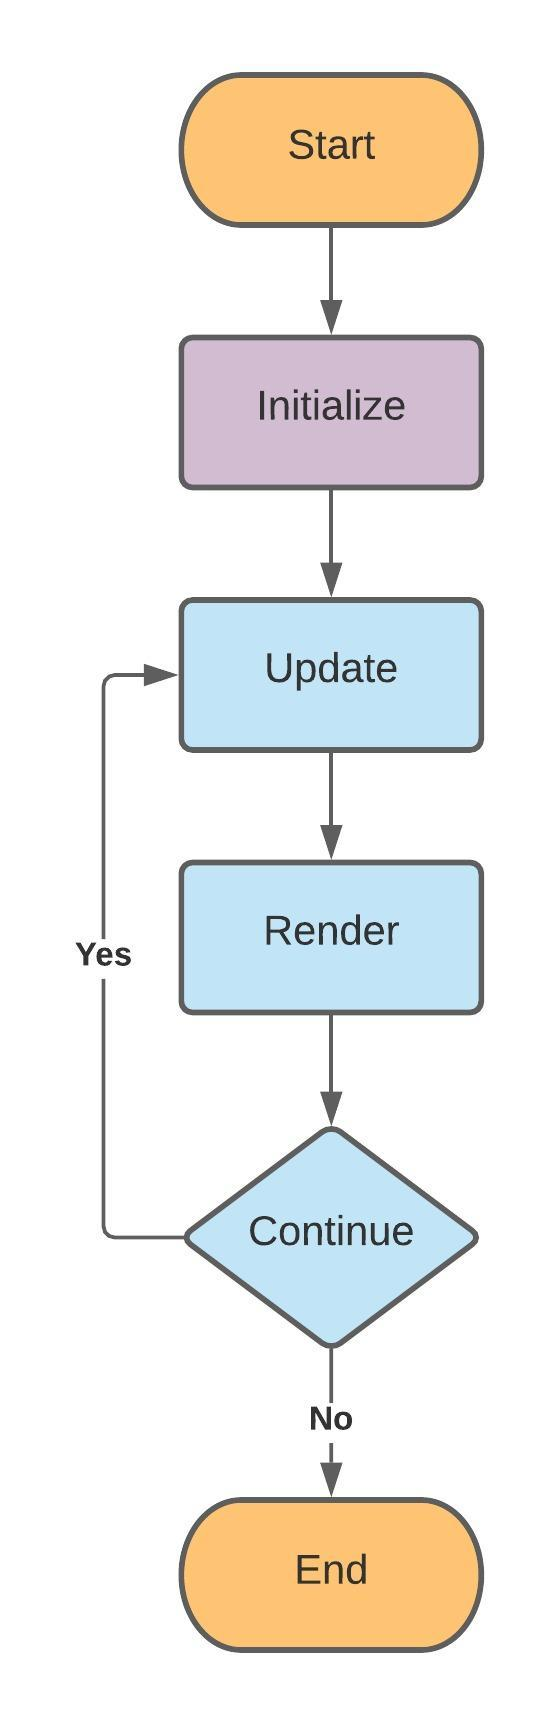
\includegraphics[scale=0.45]{visualizer_render_loop.jpg}
        \end{figure}
    \end{columns}
\end{frame}

\begin{frame}{Visualizer}
    \begin{figure}
        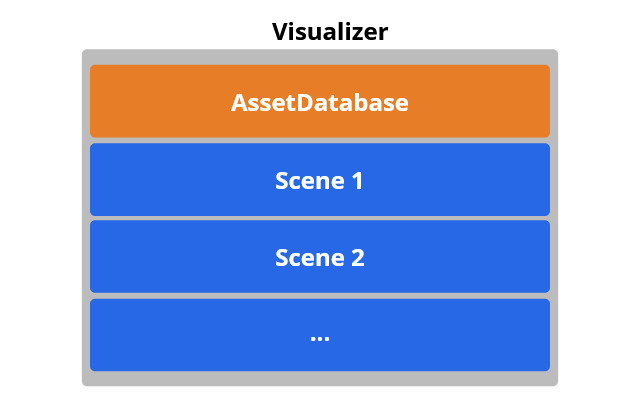
\includegraphics[scale=0.6]{visualizer_structure.jpg}
    \end{figure}
    
    \begin{itemize}
        \item Interner Aufbau ähnelt der Konfiguration.
    \end{itemize}
\end{frame}

\begin{frame}{World}
    \begin{itemize}
        \item Übernimmt die Struktur der Konfiguration.
        \item ECS (Entity-Component-System) als Basis.
        \begin{itemize}
            \item Entitäten referenzieren eine Menge an Komponenten die zum ihnen gehören.
            \item Komponente sind reine Daten und besitzen keine Logik.
            \item Logik wird in Systeme abgelagert. \\
                    Diese können den gesamten Zustand der Welt sehen und verändern.
        \end{itemize}
        \item Realisierung:
        \begin{itemize}
            \item Welt als Gruppierung von Managern.
            \item ComponentManager verwaltet Komponente und Entitäten \\
                    (Vergleichbar mit einer Datenbank).
            \item SystemManager verwaltet Systeme.
        \end{itemize}
    \end{itemize}
\end{frame}

\begin{frame}{World}
    \begin{figure}
        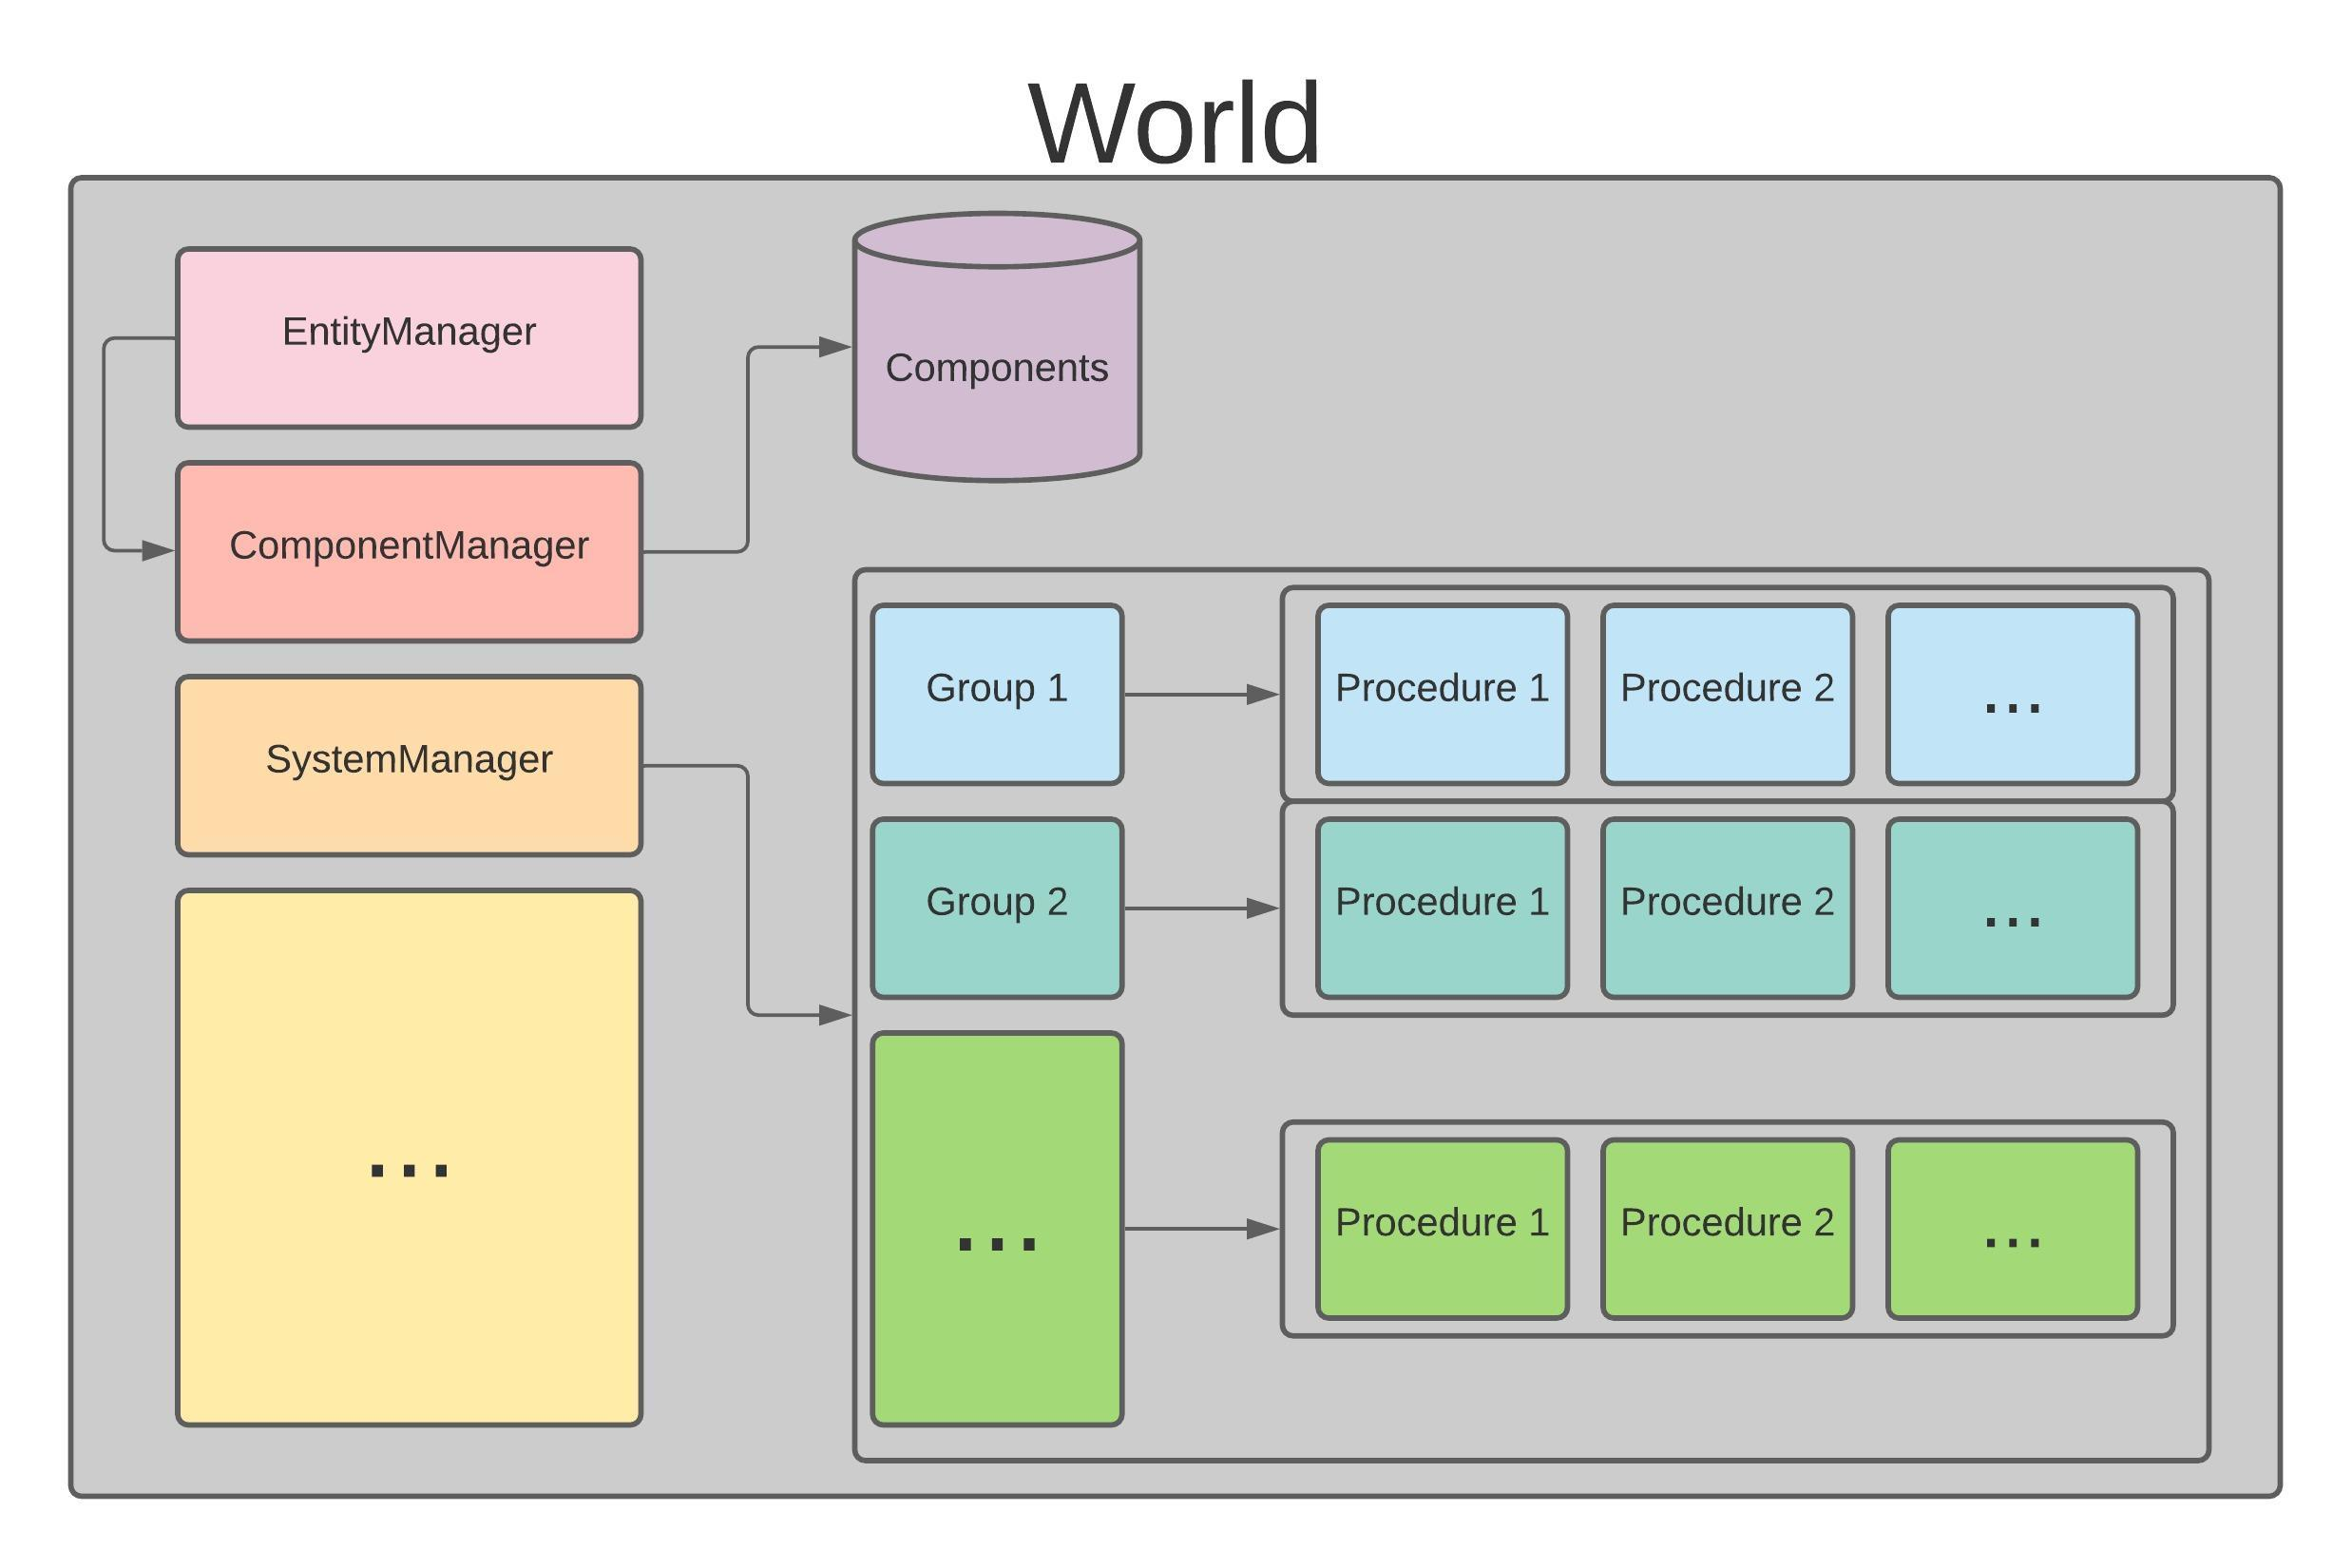
\includegraphics[scale=0.5]{world_structure.jpg}
    \end{figure}
\end{frame}

\begin{frame}[fragile]{EntityArchetype}
    \begin{lstlisting}[style=context]
struct Point {
    float x;
    float y;
    char* name;
};

// Equivalenter Archetyp.
auto archetype = EntityArchetype<std::array<float, 2>, char*>::create();

// Besser.
auto archetype = EntityArchetype<Point>::create();
    \end{lstlisting}

    \begin{itemize}
        \item Ein Archetyp beschreibt die Struktur einer Entität.
        \begin{itemize}
            \item Größe.
            \item Layout.
            \item Konstruktoren/Destruktoren.
            \item ...
        \end{itemize}
        \item Ist zur Laufzeit erweiterbar.
    \end{itemize}
\end{frame}

\begin{frame}{ComponentManager}
    \begin{figure}
        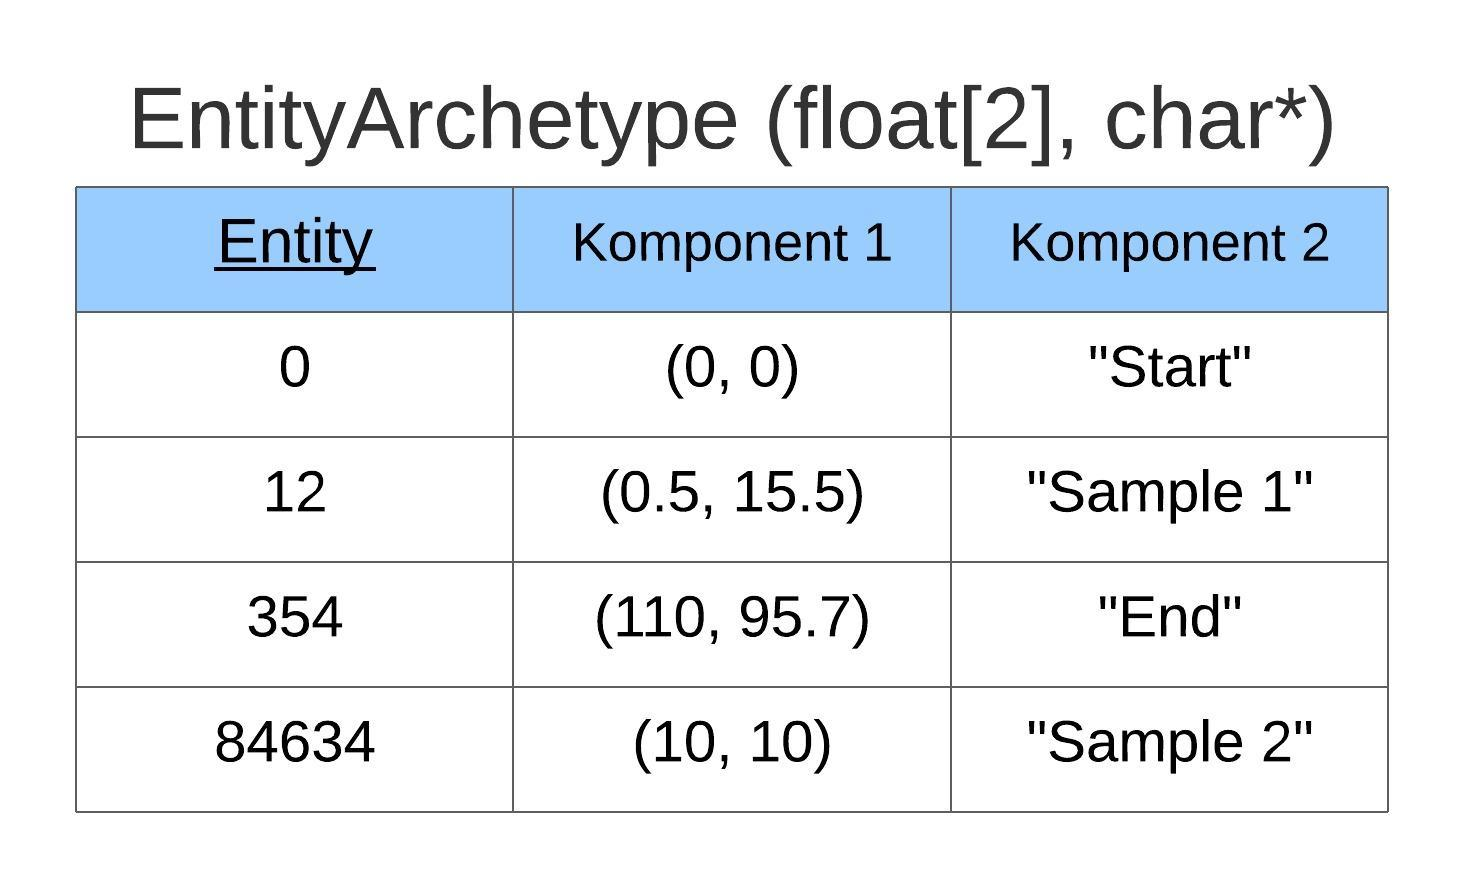
\includegraphics[scale=0.6]{entity_table.jpg}
    \end{figure}

    \begin{itemize}
        \item Der ComponentManager ist eine Datenbank.
        \item Der Archetyp identifiziert die Tabelle.
        \item Die Entität ist der Schlüssel.
        \item Man kann Querys durchführen.
    \end{itemize}
\end{frame}


\begin{frame}[fragile]{EntityQuery}
    \begin{lstlisting}[style=context]
using PointVisibility = bool;

auto point_query = EntityQuery{}.with<Point, PointVisibility>();

point_query.query(world)
    .filter<PointVisibility>([](const PointVisibility* vis) {
        return *vis;
    })
    .forEach<Point>([&](Point* p) {
        /* Verarbeite alle Points */
    });
    \end{lstlisting}

    \begin{itemize}
        \item Eine EntityQuery ist wie eine SQL-Datenbank Abfrage.
        \item Kann nach der Präsenz oder Absenz von Komponenten abfragen.
        \item Diese können dann weiter verarbeitet werden.
    \end{itemize}
\end{frame}

\begin{frame}{SystemManager}
    \begin{itemize}
        \item Eine Liste von Systeme.
        \item Werden zur Laufzeit angehängt.
        \item Werden gruppiert.
        \item Gruppen können gezielt ausgeführt werden.
        \item Eine Gruppe wird immer vollständig ausgeführt.
        \item Beispiele.
        \begin{itemize}
            \item Update
            \item Render
        \end{itemize}
    \end{itemize}
\end{frame}

\begin{frame}{Beispiel}
    \begin{figure}
        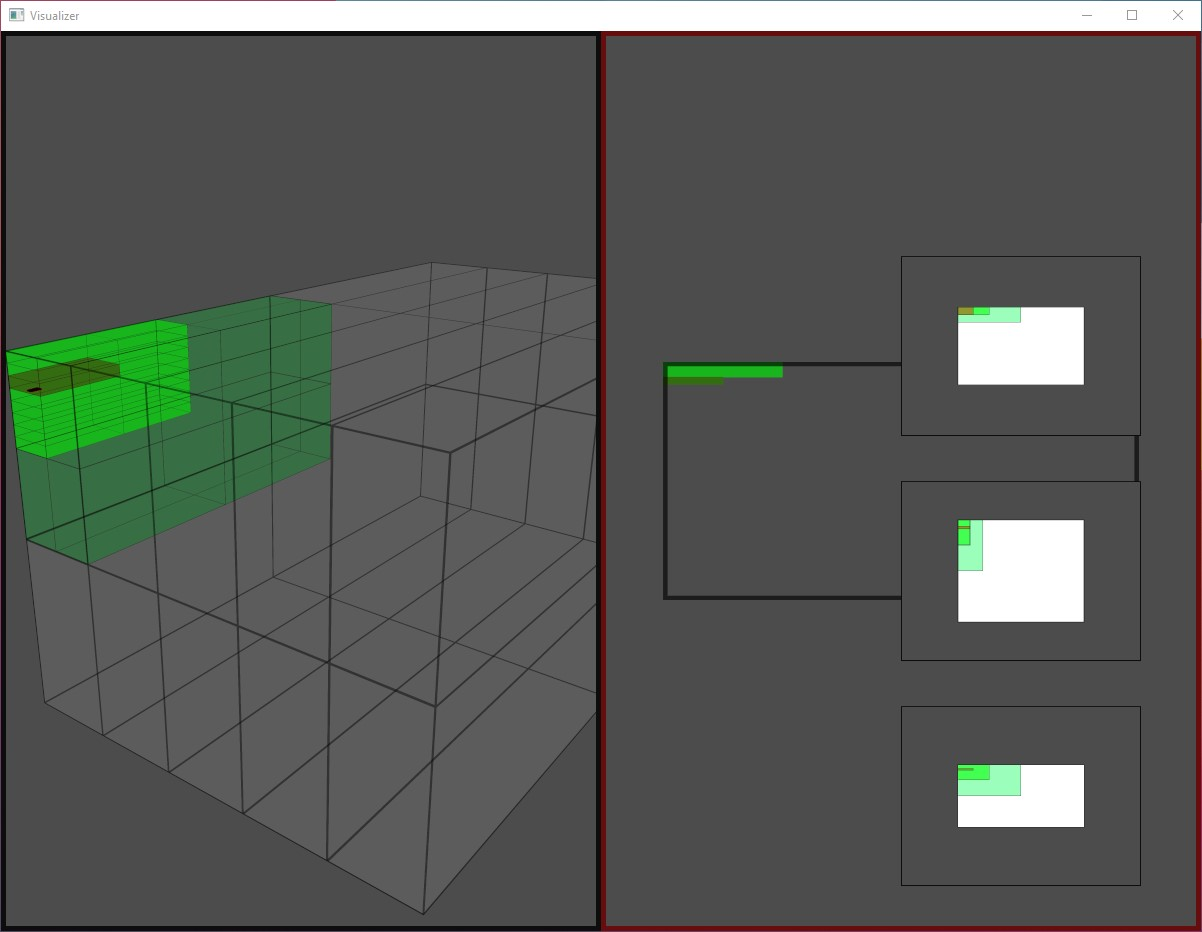
\includegraphics[scale=0.3]{visualizer.jpg}
    \end{figure}
\end{frame}

\begin{frame}{Beispiel}
    \begin{columns}
        \column{0.5\textwidth}
        \begin{itemize}
            \item View: Ein Fenster:
            \item Fenster links: MDH-View.
            \item Fenster rechts: Ausgabe-View.
            \item Kleine Fenster: Sub-Views.
            \item Quader: Layer.
            \item Die MDH-View besteht aus MDH-Layer und Thread-Layer.
        \end{itemize}
        \column{0.5\textwidth}
        \begin{figure}
            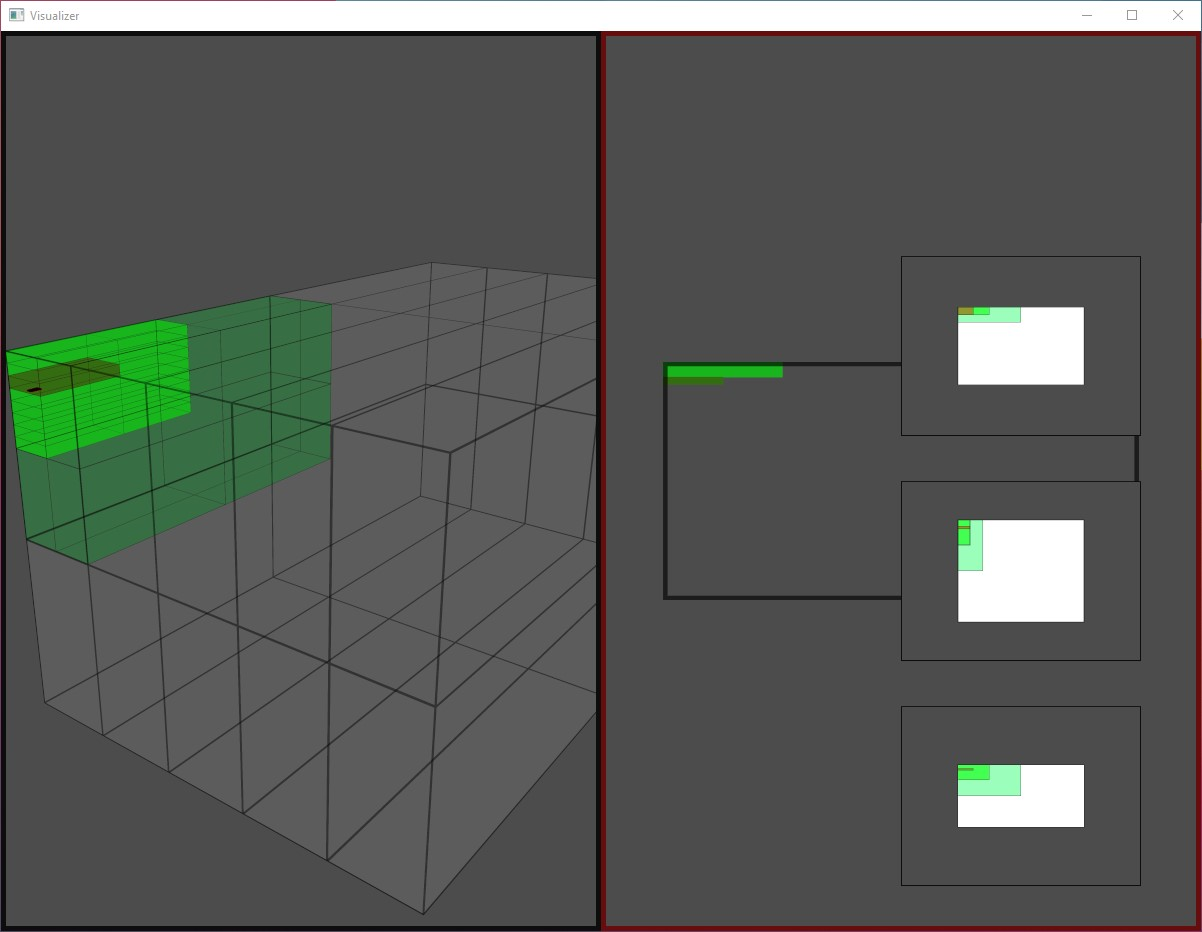
\includegraphics[scale=0.15]{visualizer.jpg}
        \end{figure}
    \end{columns}
\end{frame}

\begin{frame}{Initialisierung}
    \begin{enumerate}
        \item Konfiguration wird eingelesen.
        \item Fenster wird erzeugt.
        \item Assets werden eingelesen/erzeugt.
        \item Welt wird generiert.
        \begin{enumerate}
            \item Entitäten werden deklariert.
            \item Komponente werden initialisiert.
        \end{enumerate}
    \end{enumerate}
\end{frame}

\begin{frame}{Update}
	Der Update schritt aktualisiert den Programmzustand.
	
    \begin{enumerate}
        \item Bewegung der einzelnen Sub-Views.
        \item Bewegung der Layer.
        \item Generierung neuer Meshes.
        \item Kamerabewegung.
    \end{enumerate}
\end{frame}

\begin{frame}[fragile]{Update Ausgabeview}
    \begin{columns}
        \column{0.5\textwidth}
        \begin{table}
            \begin{tabular}{| c | c | c | c | c | c |}
                \hline
                \cellcolor{red}1 & \cellcolor{red}1 & \cellcolor{red}1 & 0 & 0 & 0 \\
                \hline
                \cellcolor{green}1 & \cellcolor{green}1 & 0 & 0 & 0 & 0 \\
                \hline
                0 & 0 & 0 & 0 & 0 & 0 \\
                \hline
                0 & 0 & 0 & 0 & 0 & 0 \\
                \hline
            \end{tabular}
            \caption{Schicht vorher}
        \end{table}

        \column{0.5\textwidth}
        \begin{table}
            \begin{tabular}{| c | c | c | c | c | c |}
                \hline
                \cellcolor{red}1 & \cellcolor{red}1 & \cellcolor{red}1 & 0 & 0 & 0 \\
                \hline
                \cellcolor{red}1 & \cellcolor{red}1 & \cellcolor{red}1 & 0 & 0 & 0 \\
                \hline
                0 & 0 & 0 & 0 & 0 & 0 \\
                \hline
                0 & 0 & 0 & 0 & 0 & 0 \\
                \hline
            \end{tabular}
            \caption{Schicht nachher}
        \end{table}
    \end{columns}
    
    \begin{enumerate}
        \item Schicht wächst um die Größe der Thread-Schicht in einer Dimension.
        \item Ein leeres Mesh wird erzeugt.
        \item Alle 2D-Projektionen der Schicht wird iteriert.
        \begin{enumerate}
            \item Es werden Rechtecke erzeugt, die die Projektion abdecken.
            \item Rechtecke werden zum Mesh hinzugefügt.
        \end{enumerate}
    \end{enumerate}
\end{frame}

\begin{frame}{Render}
    \begin{figure}
        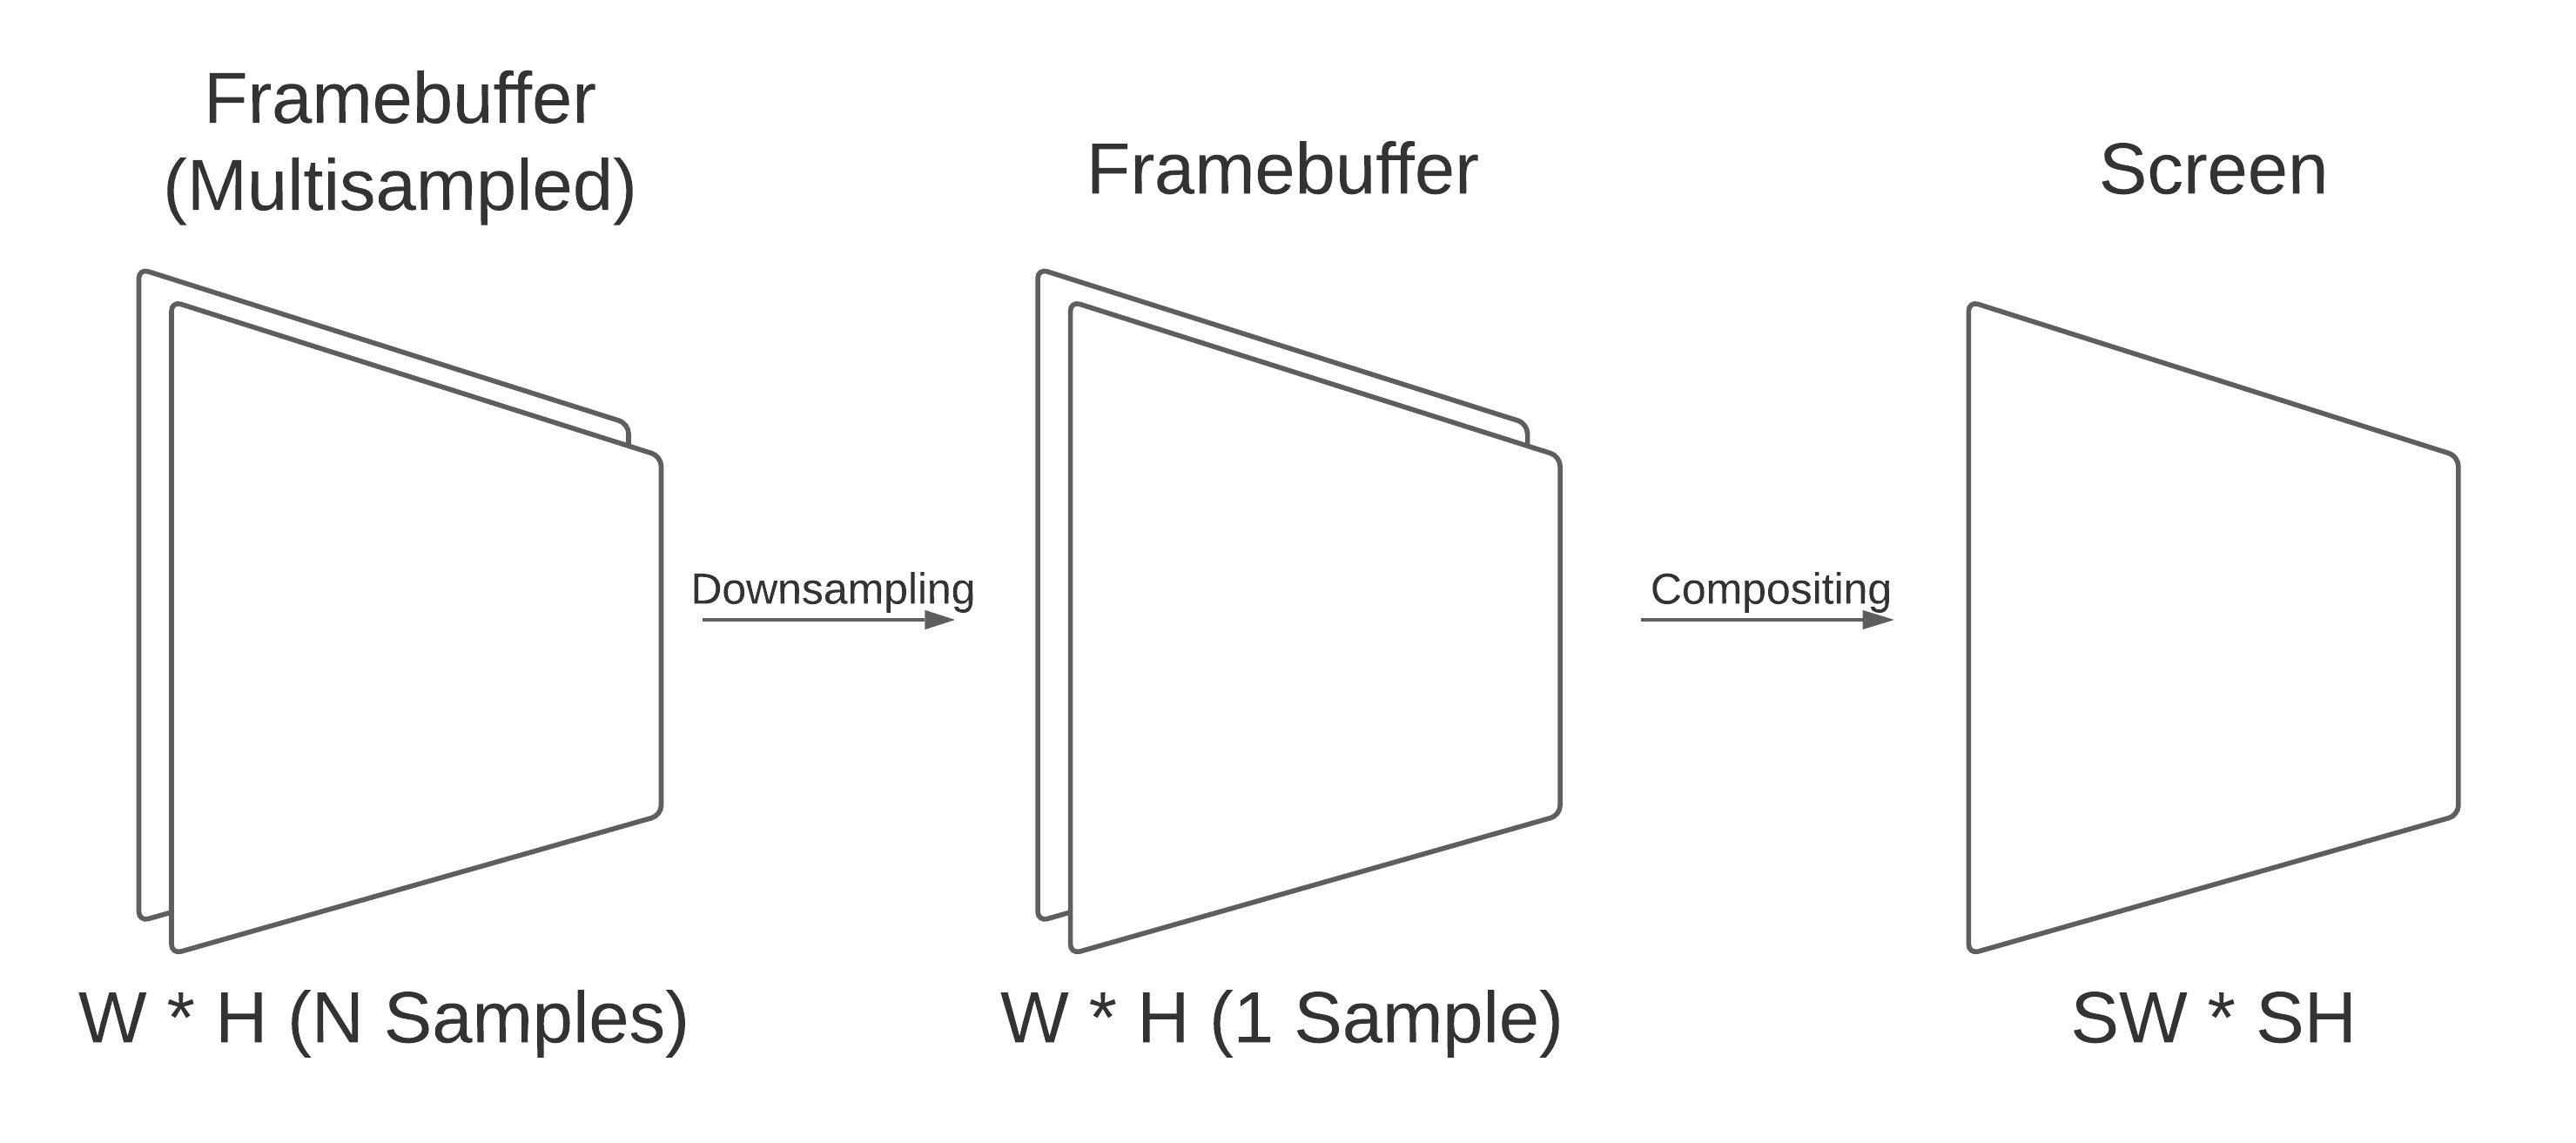
\includegraphics[scale=0.4]{render_pipeline.jpg}
    \end{figure}

    \begin{enumerate}
        \item Pro Layer 2 Framebuffer und Texturen.
        \item Meshes werden in den Framebuffer gezeichnet.
        \item Downsampling des Framebuffers.
        \item Framebuffer wird auf den Bildschirm ausgegeben.
    \end{enumerate}
\end{frame}

\section{MDH2Vis}

\begin{frame}[fragile]{MDH2Vis}
    \begin{lstlisting}[style=context]
./mdh2vis --model "path_to_model" --tps "path_to_output"
    \end{lstlisting}

    \begin{itemize}
        \item Aufgabe: Konfiguration des MDHs (MDHKonf) 
                in der neuen Konfiguration (VisKonf) überführen.
        \item Erzeugt außerdem Ressourcen die von Visualizer verwendet werden.
        \item Eingaben:
        \begin{itemize}
            \item JSON Dateien.
            \item Model: Informationen zur Darstellung der Schichten.
            \item MDH: Beschreibt die Ausgabe-View und die Sub-Views.
            \item TPS: Beschreibung des MDHs.
        \end{itemize}
        \item Model + TPS werden zum Programmstart übergeben.
        \item MDH wird beim Kompilieren eingelesen.
    \end{itemize}
\end{frame}

\begin{frame}[fragile]{MDH}
    \begin{lstlisting}[style=context]
{
    "MDH": {
        "combine operators": ["CC", "CC", "CB"]
    },
    "views": {
        "input": {
        "A": [ ["i1","i3",0] ],
        "B": [ ["i3","i2",0] ]
        },
        "output": {
        "C": [ ["i1","i2",0] ]
        }
    }
}
    \end{lstlisting}

    \begin{itemize}
        \item "MDH" beschreibt die Größe der Ausgabe-View.
        \item "views" beschreibt View-Funktionen pro Sub-View:
        \begin{itemize}
            \item Liste an Tripeln aus Lambda-Ausdrücke.
            \item Transformieren die Position im MDH in einer Position in der Sub-View.
        \end{itemize}
    \end{itemize}
\end{frame}


\begin{frame}[fragile]{MDH}
    \begin{lstlisting}[style=context]
RegisterCombineOperations sCombineOperations { "CC", "CC", "CB" }; 
std::uint32_t f_fc...(std::uint32_t i1, std::uint32_t i2, std::uint32_t i3) {
    (void)i1; (void)i2; (void)i3;
    return i1;
}
RegisterOperation<Component::X, f_fc...> s_fc... { "A" };
std::uint32_t f_67...(std::uint32_t i1, std::uint32_t i2, std::uint32_t i3) {
    (void)i1; (void)i2; (void)i3;
    return i3;
}
    \end{lstlisting}

    \begin{enumerate}
        \item Beim Start der Kompilation wir die Datei "mdh\_path.txt" eingelesen.
        \item Diese wird an "mdhunfold.py" übergeben.
        \item Dieser führt ein paar Optimierungen durch.
        \item Dann wird die Datei "MDHOps.cpp" erzeugt.
    \end{enumerate}
\end{frame}

\begin{frame}{Ablauf}
    \begin{enumerate}
        \item Model + TPS Dateien werden eingelesen und kombiniert.
        \item MDH-View wird erzeugt.
        \item Ausgabe-View wird erzeugt.
        \item Sub-Views werden erzeugt.
        \item VisKonf und Ressourcen werden erzeugt.
    \end{enumerate}
\end{frame}

\begin{frame}{MDH-View}
    \begin{enumerate}
        \item Größe wird aus der Konfiguration abgelesen.
        \item Relative Größe bezüglich des übergeordneten Layers wird berechnet.
        \item Damit kann dann die Anzahl der Iterationen pro Layer bestimmt werden.
    \end{enumerate}
\end{frame}

\begin{frame}{Ausgabe-View}
    \begin{enumerate}
        \item Größe aller Layer wird mittels "combine operations" ermittelt.
        \item Es wird errechnet wie der Layer pro Iteration wächst.
    \end{enumerate}
\end{frame}

\begin{frame}{Sub-View}
    \begin{enumerate}
        \item View-Funktionen der Sub-View werden verwendet,
                um die Größe der Layer zu bestimmen.
        \item Alle validen Indizes werden mit den View-Funktionen abgebildet.
        \item Ähnlich wie bei der MDH-View.
    \end{enumerate}
\end{frame}

\begin{frame}{VisKonf}
    \begin{enumerate}
        \item Shader und weitere Ressourcen wie Texturen und Framebuffer werden definiert.
        \item Pro View werden zwei Framebuffer und Texturen generiert, 
                wobei deren Auflösung unabhängig von der Fensterauflösung ist.
        \item Pro Layer werden drei Texturen erzeugt, um das Gitter simulieren.
        \item Layer-, Kamera- und Kontrollentitäten werden definiert.
        \item Ausgabe: visconfig.json + external\_assets
    \end{enumerate}
\end{frame}

\section{Fazit}

\begin{frame}{Fazit}
    \begin{itemize}
        \item Funktioniert sowohl mit kleine und große MDHs.
        \item Beispiel 1024x512x630 + Debug:
        \begin{itemize}
            \item Generieren der Konfiguration dauert 1–2 Minuten.
            \item Größe der erzeugten Ressourcen: 30 MB.
            \item Performance der Visualisierung ist akzeptabel.
            \item Speicherverbrauch zur Laufzeit 2–4 GB.
        \end{itemize}
        \item Noch nicht alle Eigenschaften der Konfiguration werden übersetzt.
        \item Visualisierungstool kann parallelisiert werden.
    \end{itemize}
\end{frame}

\begin{frame}
    \centering \Huge
    \emph{Danke fürs Zuhören.}
\end{frame}

\end{document}

% vi: tw=100